\section{Executing a Model-To-Model Transformation}

Having specified a correspondence metamodel for our two languages in EA; we will generate code, do some hand-written completions and execute a model-to-model transformation in this chapter.

\begin{enumerate}
\item[$\blacktriangleright$] Export your metamodels by choosing ``\texttt{Extensions/\-MOFLON::\-Ecore Addin\-/Export all to Workspace}'' in EA and push \texttt{F5} on your Eclipse Metamodel project to trigger code generation.
\end{enumerate}

If you have done everything right while modelling your TGGs in EA, code generation terminates without any error and the structure of the \texttt{gen} folder in \texttt{LearningBox\-To\-Dictionary\-Integration} resembles Fig.~\ref{fig:gen_folder}.

\begin{figure}[htbp]
\begin{center}
  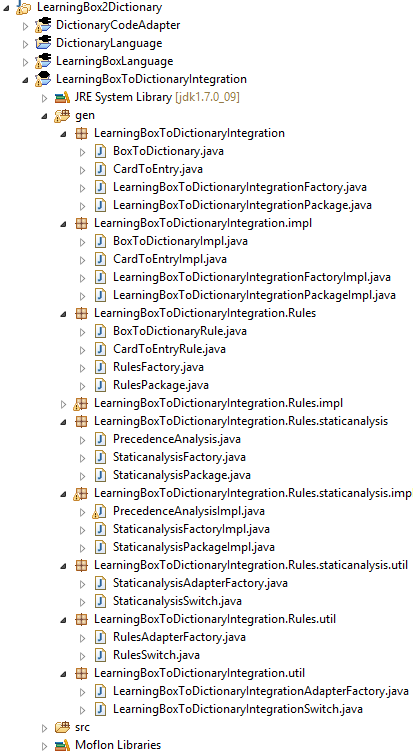
\includegraphics[width=0.6\textwidth]{pics/tggBilder/transformation/tgg22}
  \caption{\texttt{LearningBox\-To\-Dictionary\-Integration/gen} after Code Generation}  
  \label{fig:gen_folder}
\end{center}
\end{figure} 

Due to our missing \texttt{indexToLevel} implementation, the class \texttt{Card\-To\-Entry\-Rule\-Impl} is marked as faulty.
In order to make our code compile, we will create the needed class by hand:

\begin{enumerate}
\item[$\blacktriangleright$] In \texttt{LearningBox\-To\-Dictionary\-Integration/src} create the package \texttt{csp.constraints} and add a new class \texttt{IndexToLevel}.
\item[$\blacktriangleright$] Implement the class with the code provided in Fig.~\ref{fig:indexToLevel}
\end{enumerate}

\begin{figure}[htbp]
\begin{center}
  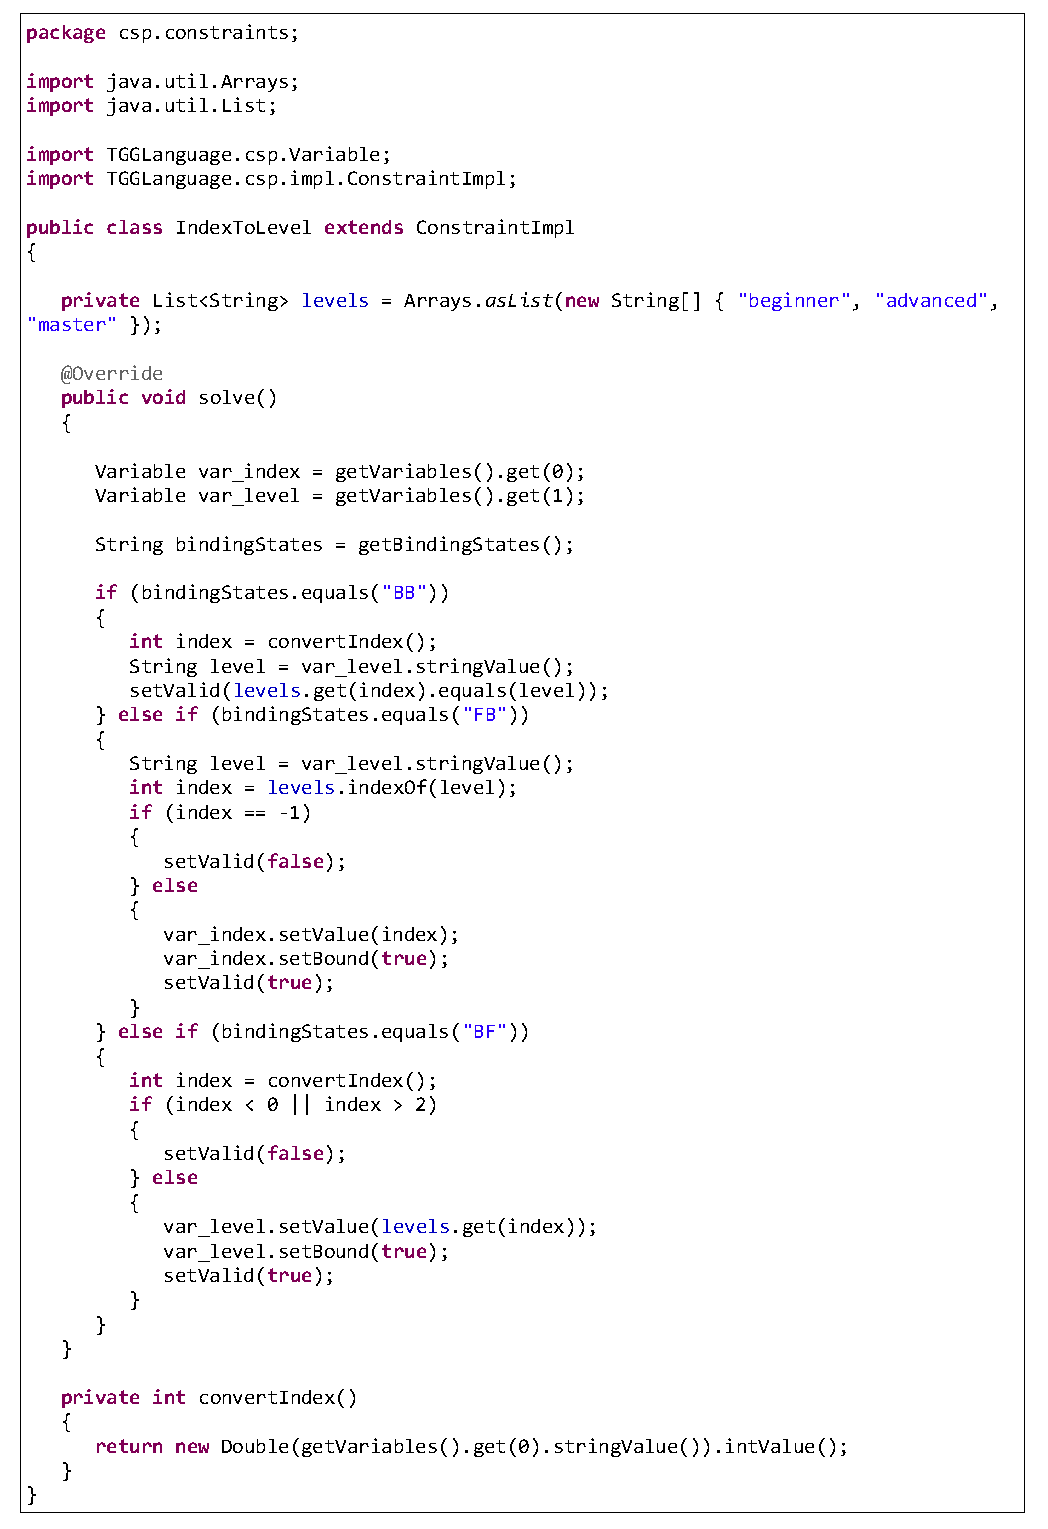
\includegraphics[width=\textwidth]{pics/tggBilder/transformation/tgg23}
  \caption{\texttt{IndexToLevel} Class implementing our Attribute Constraint}  
  \label{fig:indexToLevel}
\end{center}
\end{figure} 

After providing an implementation for our self-defined attribute constraint \texttt{indexToLevel}, the integration project \texttt{LearningBox\-To\-Dictionary\-Integ\-ration} will compile. 
At this point, we recommend you to inspect the generated code, especially the classes with \texttt{Impl}-suffix, to get a feeling how the generated code performs a transformation.

In the next steps, we will instantiate\footnote{If you are not familiar with instantiating metamodels in Ecore, then refer to Chapter \ref{sect:instance}} one of our languages, transform it to an instance of the other language and watch the simultaneous evolution of the graph triple.

\begin{enumerate}
\item[$\blacktriangleright$] Open the \texttt{Dictionary\-Language/model/Dictionary\-Language.ecore} and create a dynamic instance of \texttt{Dictionary}, name it \texttt{Dictionary.xmi} and save it under \texttt{Learning\-Box\-To\-Dictionary\-Integration/instances} (Fig.~\ref{fig:create_instance_dict}).

\begin{figure}[htbp]
\begin{center}
  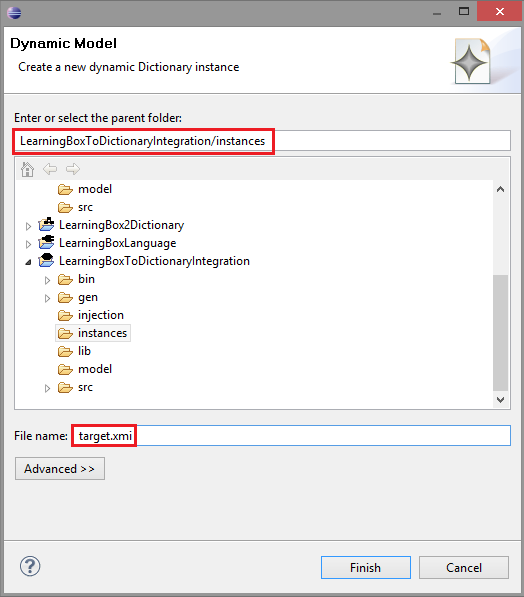
\includegraphics[width=0.5\textwidth]{pics/tggBilder/transformation/tgg24}
  \caption{Create a Dynamic Instance of \texttt{Dictionary}}  
  \label{fig:create_instance_dict}
\end{center}
\end{figure} 

\item[$\blacktriangleright$] Open \texttt{Dictionary.xmi}.
\item[$\blacktriangleright$] Set \texttt{English Numbers} as \texttt{Dictionary.title}
\item[$\blacktriangleright$] Create two \texttt{Entry} objects as child of \texttt{Dictionary}
\item[$\blacktriangleright$] Set \texttt{one : eins} as content and \texttt{beginner} as level of the first \texttt{Entry} (Fig.~\ref{fig:dictionaryxmi}).
\item[$\blacktriangleright$] Set \texttt{eleven : elf} as content and \texttt{advanced} as level of the second \texttt{Entry}.
\item[$\blacktriangleright$] Save \texttt{Dictionary.xmi}

\begin{figure}[htbp]
\begin{center}
  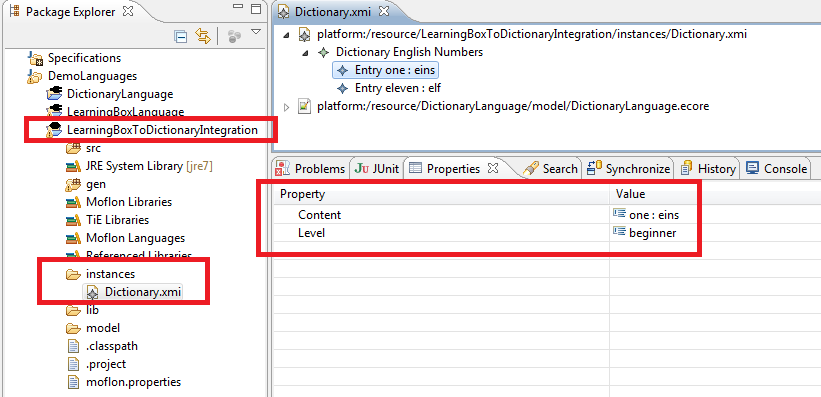
\includegraphics[width=\textwidth]{pics/tggBilder/transformation/tgg26}
  \caption{Create an Instance of \texttt{DictionaryLanguage}}  
  \label{fig:dictionaryxmi}
\end{center}
\end{figure} 

\item[$\blacktriangleright$] Create a main class \texttt{TGGMain} under \texttt{LearningBox\-To\-Dictionary\-Integration\-/src} and implement it with the code provided in Fig.~\ref{fig:tggmain}.
\item[$\blacktriangleright$] Run the class.
\item[$\blacktriangleright$] Refresh the folder \texttt{LearningBox\-To\-Dictionary\-Integration/\-instances} and check the created source and correspondence models.

\begin{figure}[htbp]
\begin{center}
  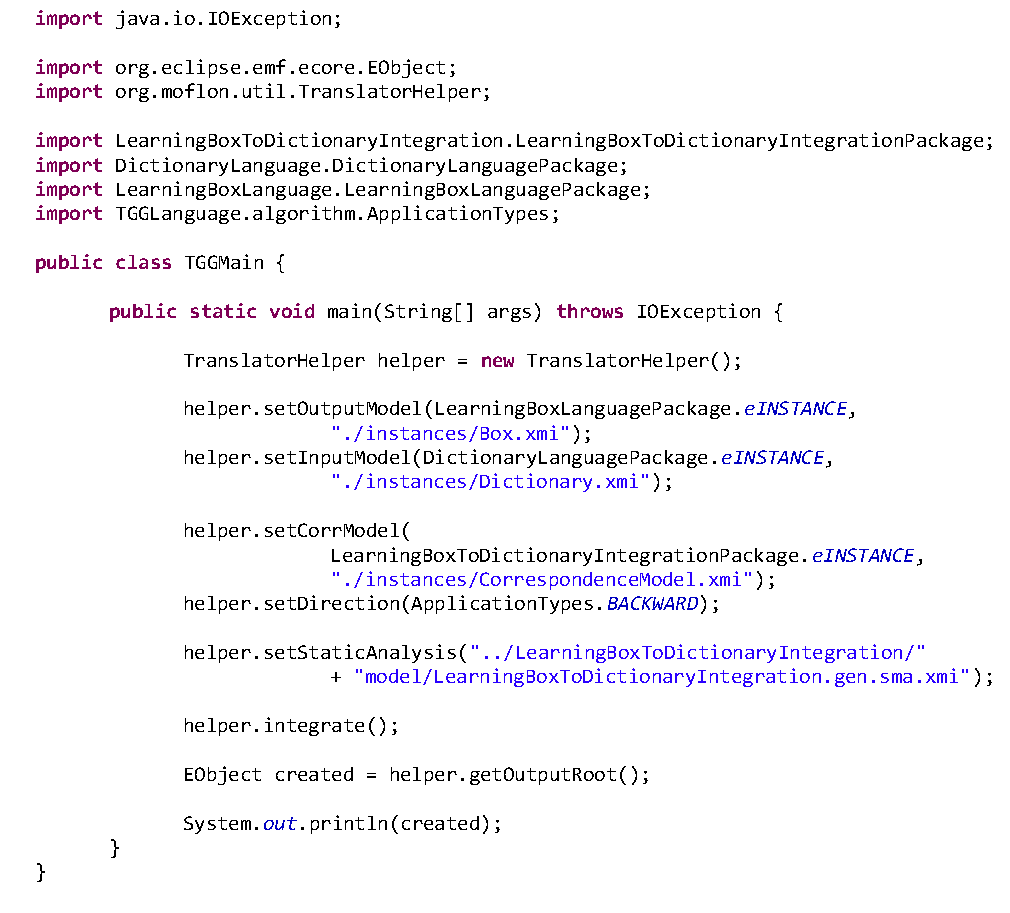
\includegraphics[width=\textwidth]{pics/tggBilder/transformation/tgg25}
  \caption{\texttt{TGGMain} Class to perform a Transformation}  
  \label{fig:tggmain}
\end{center}
\end{figure} 


\item[$\blacktriangleright$] Open \texttt{Box.xmi} in \texttt{instances} folder (Fig~\ref{fig:boxxmi}).

\begin{figure}[htbp]
\begin{center}
  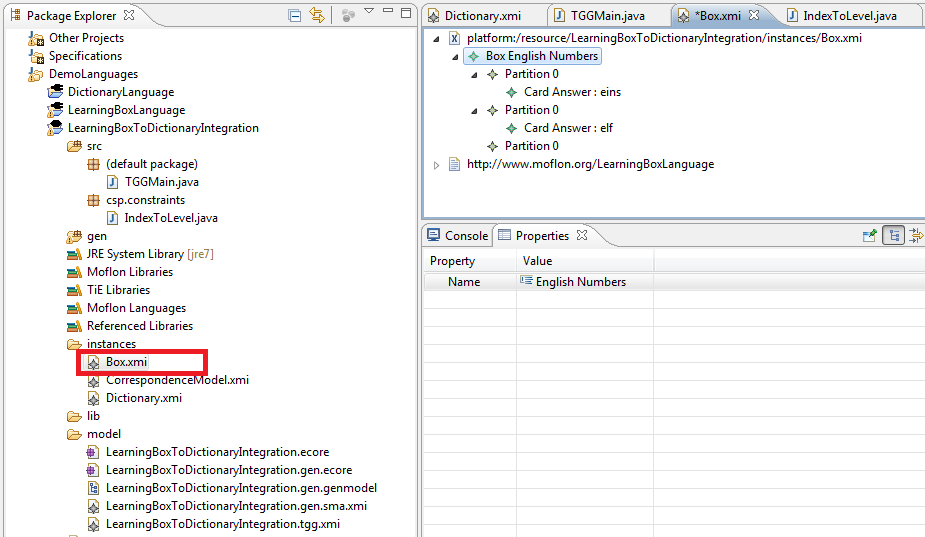
\includegraphics[width=\textwidth]{pics/tggBilder/transformation/tgg27}
  \caption{Generated Source Model \texttt{Box.xmi}}  
  \label{fig:boxxmi}
\end{center}
\end{figure} 

\end{enumerate}

You will see that our \texttt{Dictionary} is translated to a \texttt{Box} with the same name (\texttt{English Numbers}) with three underlying \texttt{Par\-ti\-tions}, as we have specified in \texttt{Box\-To\-Dictionary\-Rule}.
You will also see that the two \texttt{Entry} objects are translatlated to \texttt{Card} objects as specified in \texttt{CartToEntryRule}.
The \texttt{face} and the \texttt{back} of the \texttt{Card}s are containing a prefix and the information from the \texttt{content} of the corresponding \texttt{Entry}, e.g. \texttt{card.face = ``Question : one''} and \texttt{card.back = ``Answer : eins''}. 
The \texttt{Partition} \texttt{index}es conform also to the \texttt{Entry level}, f.i. \texttt{0} for \texttt{beginner} and \texttt{1} for \texttt{advanced}.
Being aware of the triple graph structure, we recommend you also to have a look at the created corresponcence model \texttt{CorrespondenceModel.xmi}.  

Congratulations! You have done your first model-to-model transformation with TGGs using our MOFLON tool. 
That was a \emph{backward} transformation from \texttt{Dictionary\-Language} (target model) to \texttt{Learning\-Box\-Language} (source model). 
Now, you can also edit the source model and transform it \emph{forward}:

\begin{enumerate}
\item[$\blacktriangleright$] Open \texttt{Box.xmi} and create different \texttt{Card} objects in the \texttt{Partition}s (for example, a new \texttt{Card} with \texttt{Card.face = ``Question : two''}, \texttt{Card.back = ``Answer : zwei''} in \texttt{Partition 0}). 

\item[$\blacktriangleright$] Adjust \texttt{TGGMain.java} with the code provided in Fig.~\ref{fig:tggmainforward} and run the class again.

\begin{figure}[htbp]
\begin{center}
  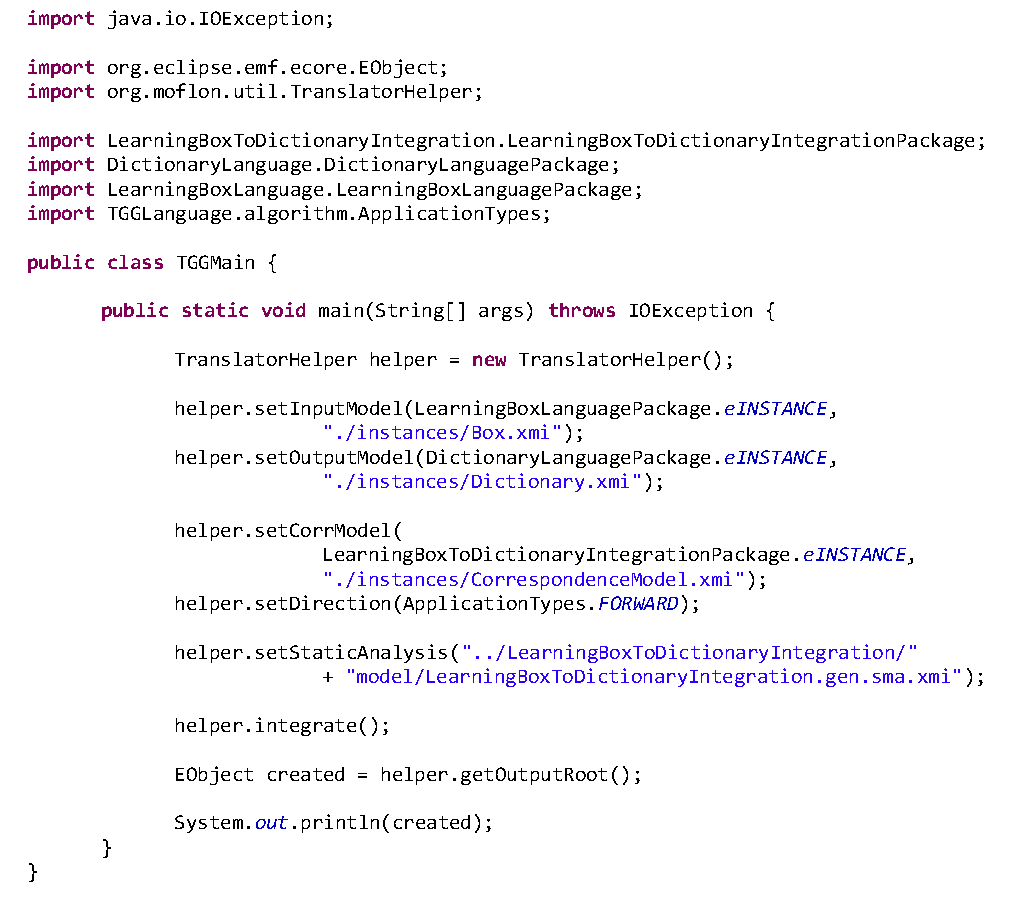
\includegraphics[width=\textwidth]{pics/tggBilder/transformation/tgg28}
  \caption{\texttt{TGGMain} for\emph{forward} transformation}  
  \label{fig:tggmainforward}
\end{center}
\end{figure} 

\end{enumerate}

You will see that your newly created \texttt{Card} objects are transformed to \texttt{Entry} objects in \texttt{Dictionary.xmi}.
That was your first forward transformation using the same generated code!

The last thing we want to show you in this chapter is our integration environment which provides you a visualisation of the graph triple in a model-to-model transformation.

\begin{enumerate}
\item[$\blacktriangleright$] Do a right click on the correspondence model \texttt{Correspondence\-Model\-.xmi} and choose \texttt{Start Integrator} from the \texttt{eMoflon} context menu (Fig.~\ref{fig:startintegrator}).

\begin{figure}[htbp]
\begin{center}
  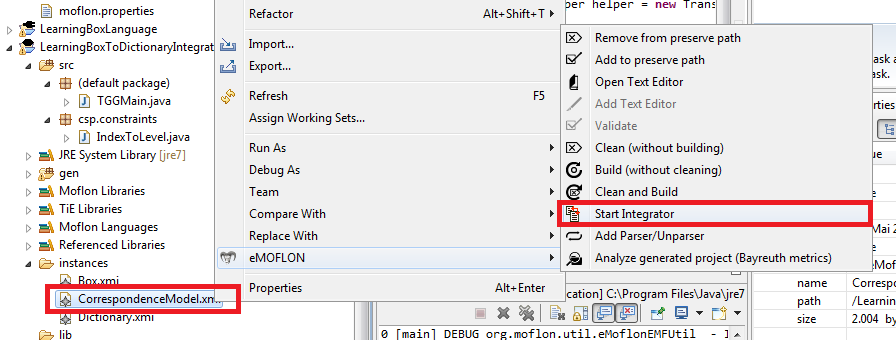
\includegraphics[width=\textwidth]{pics/tggBilder/transformation/tgg29}
  \caption{Starting the Integrator}  
  \label{fig:startintegrator}
\end{center}
\end{figure} 
\end{enumerate}

The eMoflon-Integrator window will be opened which shows you the objects from the source and target model in a treeview and visualises the links between them as depicted in Fig.~\ref{fig:emoflonintegrator}.

\begin{figure}[htbp]
\begin{center}
  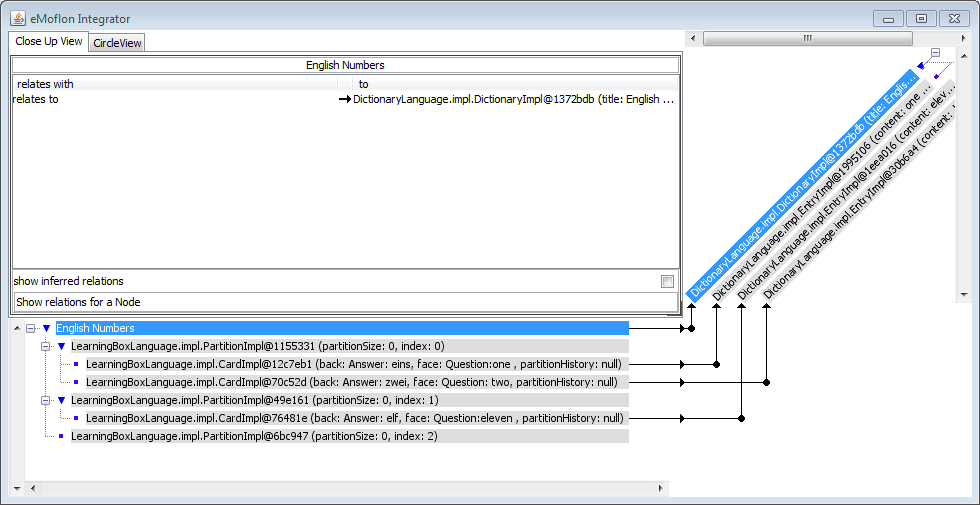
\includegraphics[width=\textwidth]{pics/tggBilder/transformation/tgg30}
  \caption{eMoflon Integrator}  
  \label{fig:emoflonintegrator}
\end{center}
\end{figure} 

